% -*- mode: latex; -*- mustache tags:  
\documentclass[10pt,twoside,english]{_support/latex/sbabook/sbabook}
\let\wholebook=\relax

\usepackage{import}
\subimport{_support/latex/}{common.tex}

%=================================================================
% Debug packages for page layout and overfull lines
% Remove the showtrims document option before printing
\ifshowtrims
  \usepackage{showframe}
  \usepackage[color=magenta,width=5mm]{_support/latex/overcolored}
\fi


% =================================================================
\title{Learning Object-Oriented Programming, Design and TDD with Pharo}
\author{Stéphane Ducasse}
\series{The Pharo TextBook Collection}

\hypersetup{
  pdftitle = {Learning Object-Oriented Programming, Design and TDD with Pharo},
  pdfauthor = {Stéphane Ducasse},
  pdfkeywords = {Introduction, programming, design, testing, Pharo, Smalltalk}
}


% =================================================================
\begin{document}

% Title page and colophon on verso
\maketitle
\pagestyle{titlingpage}
\thispagestyle{titlingpage} % \pagestyle does not work on the first one…

\cleartoverso
{\small

  Copyright 2017 by Stéphane Ducasse.

  The contents of this book are protected under the Creative Commons
  Attribution-ShareAlike 3.0 Unported license.

  You are \textbf{free}:
  \begin{itemize}
  \item to \textbf{Share}: to copy, distribute and transmit the work,
  \item to \textbf{Remix}: to adapt the work,
  \end{itemize}

  Under the following conditions:
  \begin{description}
  \item[Attribution.] You must attribute the work in the manner specified by the
    author or licensor (but not in any way that suggests that they endorse you
    or your use of the work).
  \item[Share Alike.] If you alter, transform, or build upon this work, you may
    distribute the resulting work only under the same, similar or a compatible
    license.
  \end{description}

  For any reuse or distribution, you must make clear to others the
  license terms of this work. The best way to do this is with a link to
  this web page: \\
  \url{http://creativecommons.org/licenses/by-sa/3.0/}

  Any of the above conditions can be waived if you get permission from
  the copyright holder. Nothing in this license impairs or restricts the
  author's moral rights.

  \begin{center}
    
\includegraphics[width=0.2\textwidth]{_support/latex/sbabook/CreativeCommons-BY-SA.pdf}
  \end{center}

  Your fair dealing and other rights are in no way affected by the
  above. This is a human-readable summary of the Legal Code (the full
  license): \\
  \url{http://creativecommons.org/licenses/by-sa/3.0/legalcode}

  \vfill

  % Publication info would go here (publisher, ISBN, cover design…)
  Layout and typography based on the \textcode{sbabook} \LaTeX{} class by Damien
  Pollet.
}


\frontmatter
\pagestyle{plain}

\tableofcontents*
\clearpage\listoffigures

\mainmatter

\chapter{Extending superclass behavior}
In the previous chapter we saw that inheritance allows the programmer to factor out and reuse state and behavior. As such inheritance supports the definition of class hierarchy where subclasses specialize behavior of their superclass. We saw that the method look up starts in the class of the receiver and goes up the inheritance chain. We explained that the method found by the lookup is then executed on the receiver of the initial message.
Finally we showed that a subclass can specialize and override the behavior of its superclass by defining locally a method with the same name than one method of its superclass. 

Now inheritance mechanism is even more powerful. With inheritance we can extend locally the behavior of a superclass while reusing it. It is then possible to override a method and in addition to invoke the behavior of the superclass from within the overridden method. 

We will continue to use and improve the example of file and directories.
\section{Revisiting printOn:}

\begin{figure}

\begin{center}
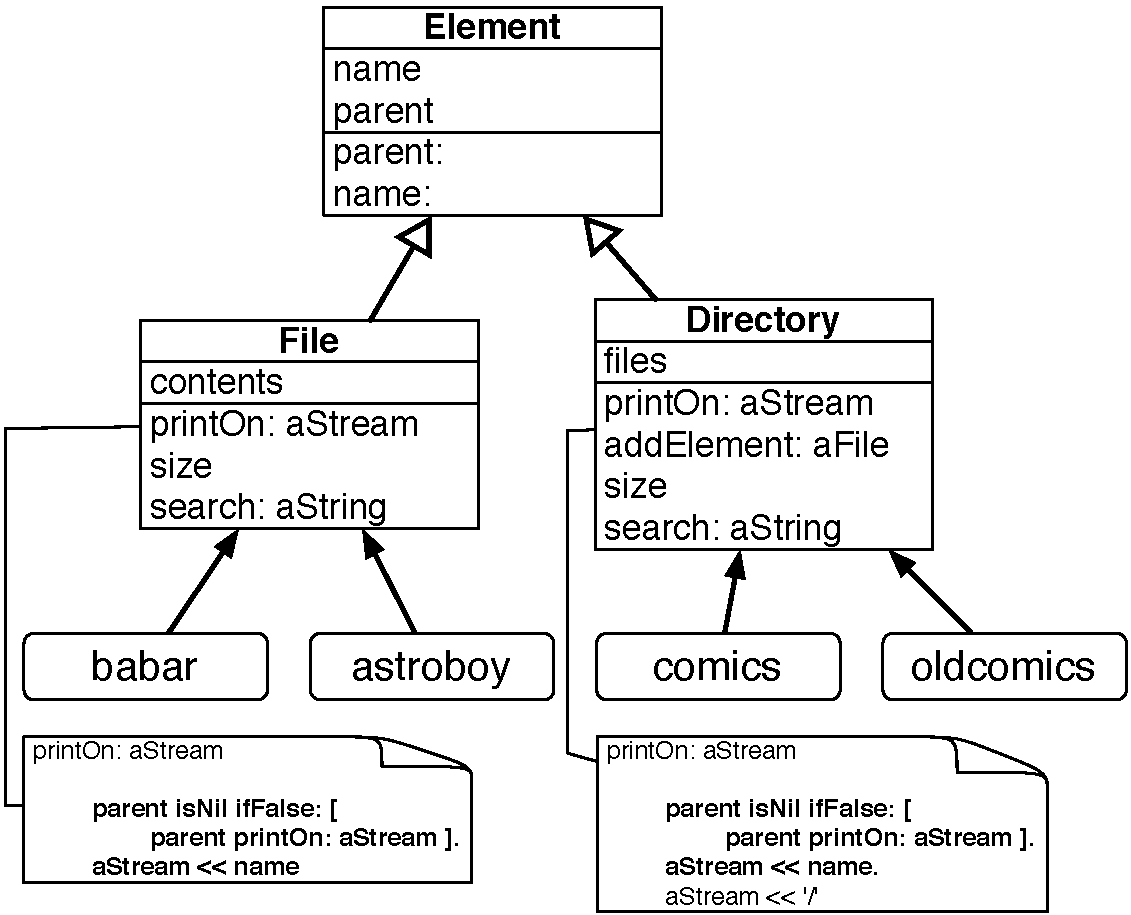
\includegraphics[width=0.65\textwidth]{/Users/ducasse/Workspace/FirstCircle/MyBooks/Bk-Writing/PharoBooks/LearningOOPWithPharoTrans/_result/pdf/Chapters/Inheritance/figures/FileDirectorySuperV0.pdf}\caption{\textcode{MFFile} and \textcode{MFDirectory} contain duplicated logic in \textcode{printOn:}.\label{fig:FileDirectorySuperV0}}\end{center}
\end{figure}


When we look at the following \textcode{printOn:} methods defined in the classes \textcode{MFDirectory} and \textcode{MFFile}
we see that there is code repetition (as shown in Figure \ref{fig:FileDirectorySuperV0}).

Here is the repeated code snippet.

\begin{displaycode}{plain}
parent isNil 
	ifFalse: [ parent printOn: aStream ].
aStream << name
\end{displaycode}

Here is the definition in the two classes: 

\begin{displaycode}{plain}
MFDirectory >> printOn: aStream
	parent isNil 
		ifFalse: [ parent printOn: aStream ].
	aStream << name.
	aStream << '/'
\end{displaycode}

\begin{displaycode}{plain}
MFFile >> printOn: aStream
	parent isNil 
		ifFalse: [ parent printOn: aStream ].
	aStream << name
\end{displaycode}

It means that if we define a new subclass we will have probably duplicate the same expression.
\section{Improving the situation}
To improve the situation above we move up the definition of the \textcode{MFFile} class because it also works for \textcode{MFElement} (as shown in Figure \ref{fig:FileDirectorySuperV1}).

\begin{displaycode}{plain}
MFElement >> printOn: aStream
	parent isNil 
		ifFalse: [ parent printOn: aStream ].
	aStream << name
\end{displaycode}


\begin{figure}

\begin{center}
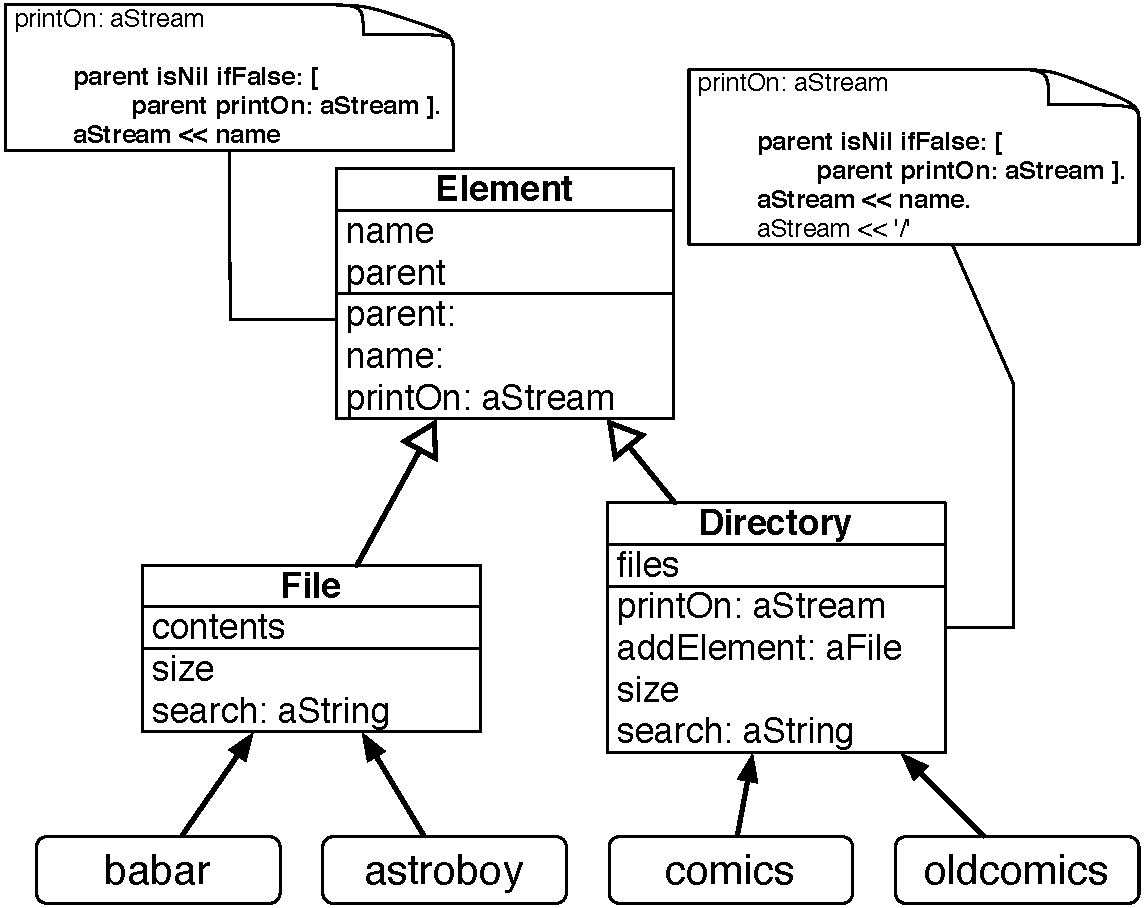
\includegraphics[width=0.65\textwidth]{/Users/ducasse/Workspace/FirstCircle/MyBooks/Bk-Writing/PharoBooks/LearningOOPWithPharoTrans/_result/pdf/Chapters/Inheritance/figures/FileDirectorySuperV1.pdf}\caption{Improving the logic (but not fully).\label{fig:FileDirectorySuperV1}}\end{center}
\end{figure}


\begin{displaycode}{plain}
MFDirectory >> printOn: aStream
	parent isNil 
		ifFalse: [ parent printOn: aStream ].
	aStream << name.
	aStream << '/'
\end{displaycode}

It means that when we will add a new subclass, this class will at least have a default definition for the \textcode{printOn:} method. 

Now the duplication of logic is not addressed. The same code is duplicated between the class \textcode{MFElement} and \textcode{MFDirectory}. What we see is that even if the method \textcode{printOn:} of class \textcode{MFDirectory} is overriding the method of its superclass, we would like to be able to invoke the method of the superclass \textcode{MFElement} and to add the behavior \textcode{aStream \textless{}\textless{} '/'}. 
\subsection{Why self does not work!}
The following definition does not work because it introduces an endless loop. Indeed, since the method lookup starts in the class of the receiver and \textcode{self} represents the receiver, it will always find the same method and will not be able to access the method of the superclass.

\begin{displaycode}{plain}
MFDirectory >> printOn: aStream
	self printOn: aStream.
	aStream << '/'
\end{displaycode}

Let us make sure that you are fully with us. Imagine that we have the following expression: 

\begin{displaycode}{plain}
| p el1 el2 |
p := MFDirectory new name: 'comics'.
el1 := MFFile new name: 'babar'; contents: 'Babar et Celeste'.
p addElement: el1.
el2 := MFFile new name: 'astroboy'; contents: 'super cool robot'.
p addElement: el2.
String streamContents: [:s | p printOn: s ]
\end{displaycode}

\begin{enumerate}
\item We get the message \textcode{p printOn: s}.
\item The method \textcode{printOn:} is looked up starting in the class of \textcode{p}, i.e., \textcode{MFDirectory}.
\item The method is found and applied on \textcode{p}.
\item The message \textcode{self printOn: aStream}  is about to be executed.
\item The receiver is \textcode{self} and represents \textcode{p}. The method \textcode{printOn: aStream} is looked up in the class of the receiver,  i.e., \textcode{MFDirectory}.
\item The same method is found in the class \textcode{MFDirectory} and the process restarts at point 3.
\end{enumerate}

In summary, we would like that while doing an override, to use the behavior we are overriding. This is possible as we will see in the following section. 


\begin{figure}

\begin{center}
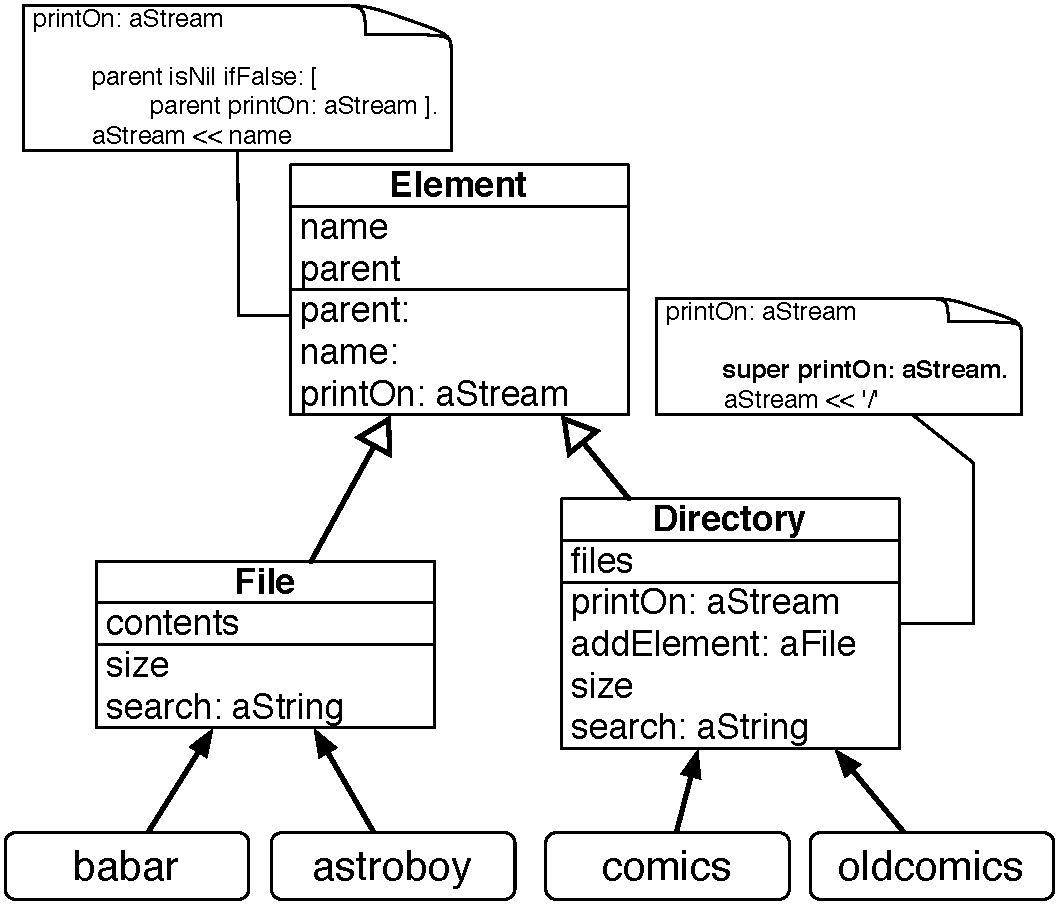
\includegraphics[width=0.65\textwidth]{/Users/ducasse/Workspace/FirstCircle/MyBooks/Bk-Writing/PharoBooks/LearningOOPWithPharoTrans/_result/pdf/Chapters/Inheritance/figures/FileDirectorySuperV2.pdf}\caption{Using \textcode{super} to invoke the overridden method \textcode{printOn:}.\label{fig:FileDirectorySuperV2}}\end{center}
\end{figure}

\section{Extending superclass behavior using super}
Let us implement the solution first and discuss it after. We redefine the method \textcode{printOn:} of the class \textcode{MFDirectory} as follows and shown in Figure \ref{fig:FileDirectorySuperV2}.

\begin{displaycode}{plain}
MFDirectory >> printOn: aStream
	super printOn: aStream.
	aStream << '/'
\end{displaycode}

What we see is that the method \textcode{printOn:} does not contain anymore the duplicated expressions with the method \textcode{printOn:} of the superclass (\textcode{MFElement}). Instead by using the special variable \textcode{super} the superclass method is invoked. Let us look at it in detail.

\begin{itemize}
\item The method \textcode{MFDirectory \textgreater{}\textgreater{} printOn:} overrides the method \textcode{MFElement}: it means that during the lookup (activated because the message \textcode{printOn:} has been sent to instances of \textcode{MFDirectory} or future subclasses), the method \textcode{MFElement \textgreater{}\textgreater{} printOn:} cannot be directly found. Indeed when a message is sent to an object, the corresponding method starts in the class of the receiver, therefore the method in \textcode{MFDirectory} is found.
\end{itemize}

\begin{itemize}
\item Using the special variable \textcode{super}, the method lookup is different than with \textcode{self}. When the expression \textcode{super printOn: aStream} is sent, the lookup does not start anymore from the class of the receiver, it starts \textit{from the superclass of the class containing the expression} \textcode{super printOn:}, i.e. \textcode{MFElement}, therefore the method of the superclass is found and executed. 
\end{itemize}

\begin{itemize}
\item Finally, \textcode{super} like \textcode{self} represents the receiver of the messages (for example an instance of the class \textcode{MFDirectory}). Therefore the method is found in the class \textcode{MFDirectory} and executed on the original object that first received the message.
\end{itemize}

Let us make sure that you are fully with us. You can compare with the previous execution simulation.

\begin{displaycode}{plain}
| p el1 el2 |
p := MFDirectory new name: 'comics'.
el1 := MFFile new name: 'babar'; contents: 'Babar et Celeste'.
p addElement: el1.
el2 := MFFile new name: 'astroboy'; contents: 'super cool robot'.
p addElement: el2.
String streamContents: [:s | p printOn: s ]
\end{displaycode}

\begin{enumerate}
\item We get the message \textcode{p printOn: s}.
\item The method \textcode{printOn:} is looked up starting in the class of \textcode{p}, i.e., \textcode{MFDirectory}.
\item The method is found and applied on \textcode{p}.
\item The message \textcode{super printOn: aStream}  is about to be executed.
\item The receiver is \textcode{super} and represents \textcode{p}. The method \textcode{printOn: aStream} is looked up in the superclass of the class containing the expression. The class containing the method is \textcode{MFDirectory}, its superclass is then \textcode{MFElement}. The lookup starts from \textcode{MFElement}.
\item The method is found in the class \textcode{MFElement} in the class.
\item The message \textcode{parent isNil} is treated on the receiver \textcode{p}.
\end{enumerate}

What we see is that using \textcode{super}, the programmer can extend the superclass behavior and reuse by involving it.

\begin{important}
\textcode{super} is the receiver of the message but when we send a message to \textcode{super} the method lookup starts in the superclass of \textbf{the class containing} the expression \textcode{super}.
\end{important}
\section{Another example}
Before explaining with a more theoritical scenario \textit{super} semantics, we want to show another example that illustrates that super expressions do not have to be the first expression of a method. We can invoke the overridden method at any place inside the overriding method.

The example could be more realistic but it shows that super expression does not have to be the first expression of a method.

Let us check the two definitions of the two methods \textcode{size} in \textcode{MFDirectory} and \textcode{MFFile}, we see that \textcode{name size} is used in both.

\begin{displaycode}{plain}
MFDirectory >> size
	| sum |
	sum := 0.
	files do: [ :each | sum := sum + each size ].
	sum := sum + name size.
	sum := sum + 2.
	^ sum
\end{displaycode}

\begin{displaycode}{plain}
MFFile >> size
	^ contents size + name size
\end{displaycode}


\begin{figure}

\begin{center}
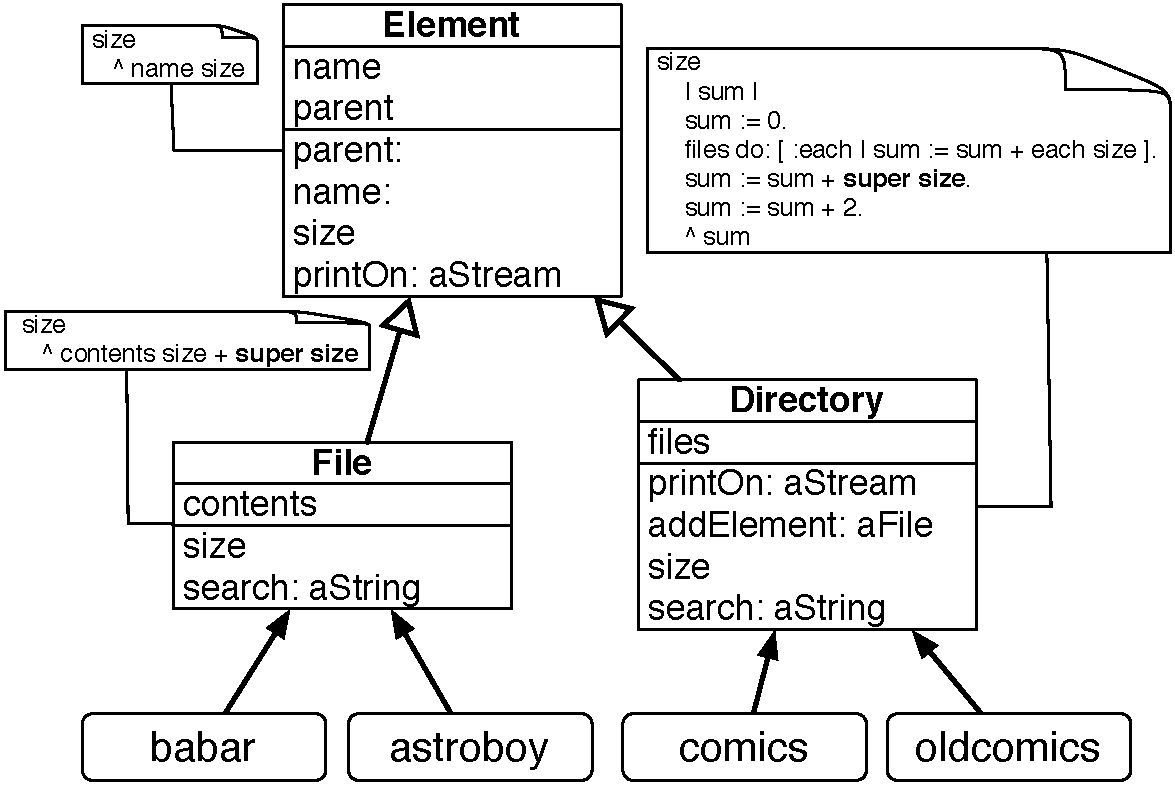
\includegraphics[width=0.65\textwidth]{/Users/ducasse/Workspace/FirstCircle/MyBooks/Bk-Writing/PharoBooks/LearningOOPWithPharoTrans/_result/pdf/Chapters/Inheritance/figures/FileDirectorySuperV3.pdf}\caption{Using \textcode{super} to invoke the overridden method \textcode{size}.\label{fig:FileDirectorySuperV3}}\end{center}
\end{figure}


What we can do is the following: define \textcode{size} in the superclass and invoke it using \textcode{super} as shown in Figure \ref{fig:FileDirectorySuperV3}. Here is then the resulting situation.

\begin{displaycode}{plain}
MFElement >> size
	^ name size
\end{displaycode}

\begin{displaycode}{plain}
MFFile >> size
	^ contents size + super size
\end{displaycode}

\begin{displaycode}{plain}
MFDirectory >> size
	| sum |
	sum := 0.
	files do: [ :each | sum := sum + each size ].
	sum := sum + super size.
	sum := sum + 2.
	^ sum
\end{displaycode}

What you see is that messages sent to \textcode{super} can be used anywhere inside in the overriding method and their results can be used as any other messages.
\section{Really understanding super}
To convince you that \textcode{self} and \textcode{super} points to the same object you can use the message \textcode{==} to verify it as follows: 

\begin{displaycode}{plain}
MFFile >> funky
	^ super == self
\end{displaycode}

\begin{displaycode}{plain}
MFFile new funky
>>> true
\end{displaycode}

\begin{important}
\textcode{super} is a special variable: \textcode{super} (just like \textcode{self}) is the receiver of the message! 
\end{important}

Now we take some time to look abstractly at what we presented so far. 
Imagine a situation as illustrated by Figure \ref{fig:LookupWithSuperInSuperclassMethodThreeClasses}.

\begin{displaycode}{plain}
A new bar
>>> ...
C new bar
>>> ...
D new bar
>>> ...
\end{displaycode}
\subsection{Solution }

\begin{figure}

\begin{center}
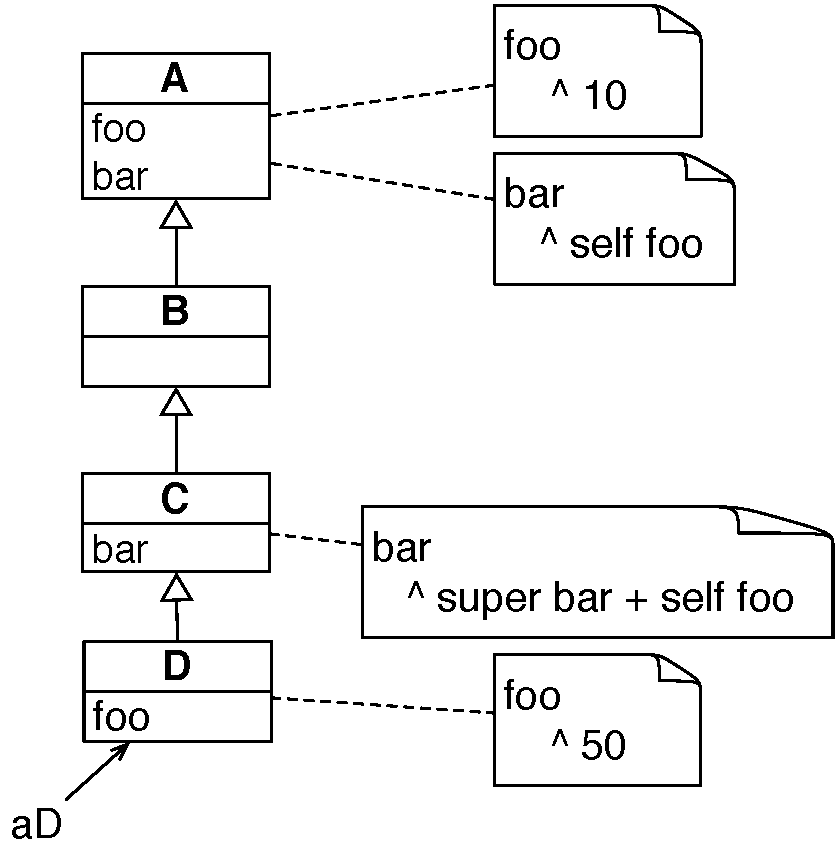
\includegraphics[width=0.35\textwidth]{/Users/ducasse/Workspace/FirstCircle/MyBooks/Bk-Writing/PharoBooks/LearningOOPWithPharoTrans/_result/pdf/Chapters/Inheritance/figures/LookupWithSuperInSuperclassMethodThreeClasses.pdf}\caption{Example to understand \textcode{super}.\label{fig:LookupWithSuperInSuperclassMethodThreeClasses}}\end{center}
\end{figure}


The solutions are the following ones:

\begin{displaycode}{plain}
A new bar
>>> 10
C new bar
>>> 20
D new bar
>>> 100
\end{displaycode}

Let us examine the evaluation of the message \textcode{aD bar}: 

\begin{enumerate}
\item \textcode{aD}'s class is \textcode{D}.
\item There is no method \textcode{bar} in D.
\item The method look up in \textcode{C}. The method \textcode{bar} is found.
\item The method \textcode{bar} of \textcode{C} is executed.
\item The message \textcode{bar} is sent to \textcode{super}.
\item \textcode{super} represents \textcode{aD} but the lookup starts in the superclass of the class containing the expression \textcode{super} so it starts in \textcode{B}.
\item The method \textcode{bar} is not found in \textcode{B}, the lookup continues in \textcode{A}.
\item The method \textcode{bar} is found in \textcode{A} and it is executed on the receiver i.e., \textcode{aD}.
\item The message \textcode{foo} is sent to \textcode{aD}.
\item The method \textcode{foo} is found in \textcode{D} and executed. It returns 50. 
\item Then to finish the execution of method \textcode{bar} in \textcode{C}, the rest of the expression \textcode{+ self foo} should be executed.
\item Message \textcode{self foo} returns 50 too, so the result returns 100. 
\end{enumerate}

\begin{important}
The difference between \textcode{self} and \textcode{super} is that when we send a message to \textcode{super} the method lookup starts in the superclass of the class containing the expression \textcode{super}.
\end{important}
\section{Conclusion}
In this chapter we saw that inheritance also supports the possibilities to override a method and from this overriding method to invoke the overridden one. This is done using the special variable \textcode{super}. 
\textcode{super} is the receiver of the message like \textcode{self}. The difference is that the method lookup is changed when messages are sent to \textcode{super}. The method is looked up in the superclass of the class containing the message sent to \textcode{super}. 


% lulu requires an empty page at the end. That's why I'm using
% \backmatter here.
\backmatter

% Index would go here
\bibliographystyle{abbrv}
\bibliography{others.bib}
\end{document}
